\section{Testing} \label{Section:Testing}
Testing is necessary in order to ensure that all the required functionality is achieved by the system. With the agile approach that has been adopted, testing plays a key role and the as a result the development and testing process are essentially intertwined. Unit tests were performed throughout the development process upon the completion of each component and integration testing was performed when these components were integrated into the rest of the system. The testing procedures carried out that both the functional and non-functional requirements of the system were met. Additionally user testing was carried to ensure that the system was usable by the general public. These tests have been documented and discussed in this section.


\subsection{Unit Testing}
Unit testing is a software development process in which the smallest testable parts of an application, called units, are individually and independently scrutinised for proper operation \cite{TechTarget:UnitTesting}. Through unit testing, the developer can test each aspect of the system at a micro level before each component is integrated into the system. These unit tests were mostly dictated by the functional and non-functional requirements of the system to ensure that the component satisfied all the requirements. Throughout this process, white-box testing has been used along with some black-box testing to ensure expected behaviour is provided by the system. Table \ref{table:Unit_Testing} below discusses the tests carried out as part of unit testing by stating the expected behaviour and the actual behaviour.

\begin{longtable}{@{}p{0.04\textwidth}p{0.27\textwidth}p{0.27\textwidth}p{0.28\textwidth}@{}}
	\toprule
	F\# & Description & Input & Result \\ \midrule
	
	2 & Sign up using email & Form data filled in by user & \textcolor{PassGreen}{Pass}: new account is created and the user is logged in\\
	
	2 & Sign up using Facebook oAuth & User clicks Facebook oAuth service link to provide Frisk with authentication credentials & \textcolor{PassGreen}{Pass}: The users credentials are returned by Facebook \\
	
	2 & Sign up using Google oAuth & User clicks the Google oAuth service link to provide Frisk with authentication credentials & \textcolor{PassGreen}{Pass}: The users credentials are returned by Google \\
	
	2 & Sign up using multiple services with same email & The user chooses to authenticate with one service then another with the same email & \textcolor{PassGreen}{PASS}: The first time an account is created but any new services after that are just associated with the existing account \\

	2 & Login using valid email and password & User provides their email and password using the login form & \textcolor{PassGreen}{Pass}: The user is successfully authenticated and redirected to the homepage \\
	
	2 & Login using invalid email or password & User provides their email and password using the login form &  \textcolor{PassGreen}{Pass}: An error is returned to the user notifying them that their credentials are invalid \\
	
	2 & Login using an oAuth service provider & User clicks one of the oAuth service links to provide Frisk with authentication credentials & \textcolor{PassGreen}{Pass}: The users credentials are returned by the service and the associated user is authenticated then redirected \\
	
	2 & Logging out of the system & The user clicks the logout link after authenticating with any of the services & \textcolor{PassGreen}{Pass}: The user is logged out and redirected to the homepage. \\
	
	3 & Creating location using postcode & The user clicks new location and enters their postcode to find the location then presses save & \textcolor{PassGreen}{Pass}: The address is automatically resolved for the user and clicking save registers the location \\
	
	3 & Creating location using current location & The user chooses current location from the new location dialogue & \textcolor{PassGreen}{Pass}: The users current location is retrieved and the address is automatically found which can be saved \\
	
	3 & Creating location with invalid postcode & The user enters a postcode that doesn't exist & \textcolor{PassGreen}{Pass}:  An error is returned to the user, prompting them to try again \\
	
	
	4 & Deleting an unused location & Clicking the delete button on an unused location & \textcolor{PassGreen}{Pass}: The location is deleted and a success notification is presented \\
	
	4 & Deleting an in-use location & Clicking the delete button on a location currently in use & \textcolor{PassGreen}{Pass}: The location is not deleted and the user is presented with an error stating the location is in use \\
	
	5 & Creating an item & The user completes the input form for creating an item and submits it & \textcolor{PassGreen}{Pass}: The location is created and the user is redirected to the items page on the dashboard where the item is listed under private\\
	
	5 & Creating an item with and without optional information & The user enters additional information or leaves it out & \textcolor{PassGreen}{Pass}: The item is created either way and the user is redirected to the items page \\
	
	6 & Editing an existing item & Clicking the edit link, changing the item details and pressing save & \textcolor{PassGreen}{Pass}: The item details are updated in the database and the user is redirected \\
	
	7 & Deleting an item & Clicking the delete button on an item & \textcolor{PassGreen}{Pass}: The item is soft deleted and removed from the user page \\
	
	7 & Deleting an item with resources & Clicking the delete button on an item with resources & \textcolor{PassGreen}{Pass}: The item is soft deleted along with associated resources and theft records \\
	
	8 & Reporting an item as lost or stolen & The user selects a location and click the report as lost or stolen button & \textcolor{PassGreen}{Pass}: The item is immediately marked as lost or stolen and becomes available on the public search. \\
	
	9 & Marking an item as recovered & The user clicks the mark as recovered button & \textcolor{PassGreen}{Pass}: The item is immediately removed from public search and made private \\
	
	10 & Uploading images & The user uploads an image by dragging it onto the upload area and by choosing using the choose file menu & \textcolor{PassGreen}{Pass}: The image is successfully uploaded and stored as a private image \\
		
	10 & Uploading a file other than images & The user uploads a file by dragging it onto the upload area and by choosing using the choose file menu & \textcolor{PassGreen}{Pass}: The resource is uploaded and stored as type 'other' \\
	
	11 & Editing an image & Clicking edit on a resource when there are multiple public resources & \textcolor{PassGreen}{Pass}: A dialogue pops up allowing the user to edit the alias and whether the image is public or private \\
	
	11 & Editing the last image & Clicking the edit button on the last public image & \textcolor{PassGreen}{Pass}: This time a dialogue pops up but the user can only edit the alias and is not allowed to make this image private \\
	
	
	11 & Editing a resource other than image & Clicking the edit button on the resource & \textcolor{PassGreen}{Pass}: An edit dialogue pops up allowing the user to edit only the alias as non-image files can't be made public \\
	
	12 & Deleting a resource when there are many public resources & Clicking the delete button on a resource & \textcolor{PassGreen}{Pass}: The resource is deleted and a success notification is presented to the user \\
	
	12 & Deleting resources when there is only one public resource & Clicking the delete button on a resource & \textcolor{PassGreen}{Pass}: The resource is deleted if it isn't the last public resource, otherwise an error notification is presented \\
	
	13 & Search for items as guest and registered user & Search for an item by entering a query in the search bar & \textcolor{PassGreen}{Pass}: In both cases the user is redirected to the search page where any matching results are displayed \\
	
	13 & Search for an item using name & Enter the name of an item in the search bar & \textcolor{PassGreen}{Pass}: The user is redirected to the search page and any items with a similar name are displayed \\
	
	13 & Search for an item using unique identifier & Enter the unique identifier of an item in the search bar & \textcolor{PassGreen}{Pass}: The user is redirected to the search page and any results where the identifier contains the query are displayed \\
	
	14 & Exploring items & Clicking the around me link in the navigation bar & \textcolor{PassGreen}{Pass}: The users location is requested and they're redirected to the explore page which lists all items within 20km \\

	14 & Sorting explore results & Choose a sorting option from the sort by drop down menu & \textcolor{PassGreen}{Pass}: The page is refreshed and the results are updated and displayed in the request order \\
	
	14 & Exploring item on desktop & Using a desktop site, click around me in the navigation bar & \textcolor{PassGreen}{Pass}: The user is redirected to the explore page where 60\% of the page shows the result tiles and the other 40\% shows a map \\
	
	14 & Exploring items on mobile device & Using a mobile device, click around me in the collapsible navigation & \textcolor{PassGreen}{Pass}: The user is redirected to the explore page but only the tile view is presented \\
	
	15 & Viewing an item & Clicking a result on the search or explore page & \textcolor{PassGreen}{Pass}: Clicking a result brings up a modal with more details about the item and a message owner link \\
	
	16 & Message owner link for guests & Clicking the message owner link on the view item modal as a guest & \textcolor{PassGreen}{Pass}: The user is redirected to the login page \\
	
	16 & Message owner link for authenticated users & Clicking the message owner link on the view item modal whilst logged in & \textcolor{PassGreen}{Pass}: The user is redirected to the create message page with certain fields populated automatically \\
	
	17 & Messaging owner of recovered item & Click message owner or visit the create message  url for an item after it has been recovered & \textcolor{PassGreen}{Pass}: The user is redirected back to the inbox as you cannot contact a person when there is nothing to inform the user about \\
	
	17 & Attempting to send a message for your own item & Click message owner for an item that you've reported as stolen & \textcolor{PassGreen}{Pass}: The user is redirected back to the messages page as they cannot message themselves \\
	
	17 & Messaging system & Click the messages link in the normal navigation or the dashboard sidebar & \textcolor{PassGreen}{Pass}: The user is redirected to their inbox where the messages are displayed in a table like format similar to emails \\

	17 & Viewing a sent or received message & Click a message on the messages page & \textcolor{PassGreen}{Pass}: The user is redirected to the view message page and the message is marked as read if the user is the recipient \\
	
	18 & Replying to messages & Click the reply link next to a message on the inbox page or view message page & \textcolor{PassGreen}{Pass}: The user is redirected to the reply message page where they can enter a message and press send to reply \\
	
	18 & Attempting to reply to your own message & Click reply to a message that was created by the active user & \textcolor{PassGreen}{Pass}: The user is simply redirected back to the inbox for performing an invalid operation \\
	
	19 & Delete a received message & Click delete next to a received message on the inbox page & \textcolor{PassGreen}{Pass}: The message is deleted only for the recipient but not for the sender \\
	
	19 & Deleting a sent message & Click delete next to a sent message on the sent messages page & \textcolor{PassGreen}{Pass}: The message is deleted for the sender but not for the recipient \\ \bottomrule
	
	\caption{Unit Tests Carried out to Verify Functional Requirements}
	\label{table:Unit_Testing}
\end{longtable}

\subsubsection{Validation Testing}

In addition to the unit testing carried out, which verified if the functional requirements were met, testing on requests for each of these unit was also carried out. This process involved making sure the validation rules for each of the requests were correct and the errors returned for invalid requests were appropriate. In order to entirely sure, valid, invalid and boundary inputs were tested for each field on each form for every single component before it was integrated into the system. Additionally, empty forms were submitted and forms without valid csrf tokens were also submitted to test the response as well as any errors generated.

\begin{lstlisting}[language=php]
	$deleted = $location->items()->count() == 0 && $location->stolenRecords()->count() == 0 && $location->delete();
\end{lstlisting}

Further to form validation, other measures were put in place which validated requests such as deletion. These verified that a delete request would not result in database inconsistency and thus had to be tested as well. For example, the line of code above checks to see if a location is assigned to any items before deleting it and had to be tested.

\subsubsection{Permission Testing}
Protecting the users and their data is important and any measures put in place need to be tested thoroughly. After development of a component, permission testing was carried out on the component to guarantee absolute security. The permission testing checked verified that certain pages were only available to authorised users whereas others are available to everyone. This functionality was provided by the authentication middleware but was tested for each page to make sure it was being applied.

\begin{lstlisting}[language=php]	
	$success = $item && $item->user_id == Auth::user()->id;
\end{lstlisting}

In addition to verifying just permission to view a page, it was also necessary to verify request on a per user basis. This means checking that a user requesting to perform an operation is actually allowed to perform that operation. For example, only the owner of an item is allowed to edit or delete an item and anyone else attempting to an item not belonging to them should be dealt with accordingly. The line of code above ensures that only the owner of the item can access the edit item page, otherwise the user is redirected to another page. Features like this exist through the system and were also part of the permission testing process.

\subsection{Integration and System Testing}
Integration testing is a logical extension of unit testing. In its simplest form, two units that have already been tested are combined into a component and the interface between them is tested \cite{MSDN:IntegrationTesting}. As the major functionality of each component was completed, the component could now be integrated into the system so that it may work along the other components. Once integrated, integration testing could be carried out to ensure that each  individual component functioned alongside other components, that it may have relied on, without resulting in errors. Integration testing prevents errors from propagating into the subsequently implemented components. Every time a component was integrated, all the unit tests for that components were run again to verify its functionality. Any errors that occurred were fixed and the tests were rerun before moving onto the next component. 

System testing is most often the final test to verify that the system to be delivered meets the specification and its purpose \cite{ISTQB:SystemTesting}. In system testing the behaviour of whole system is tested as defined by the scope of the development project or product \cite{ISTQB:SystemTesting}. However, system testing was carried out for the project as the system was developed as well as at the end - This means that as each component was developed and integrated, thorough testing was done on the component integrated, any other components it affected as well as the general functionality of the system. In comparison to unit and integration testing which verify that functional requirements are met, system testing verifies both functional and non-functional requirements of the system. Additionally, at the end of the development process, a comprehensive and thorough system test was carried out using multiple user accounts. These tests followed the same convention and produced the same results as the unit tests. Any errors that occurred were patched on the go and the testing was done all over again.

\subsection{User Acceptance Testing}
The entire system relies on a stable and growing user base, without the users the system would be rendered useless. With user experience being such an integral part of the system, it was important to identify what the users opinions of the system. This data could be used to identify the strength and the weaknesses of the system at various stages of prototyping. A number of users were consulted after being given access to the system at various stages of development in order to identify any issues that users may have with the system so that these could potentially be solved in the next iteration of the system.

At various stages of the system the users were given surveys along with a list of tasks to complete. Once the users completed each task, they would answer the questions corresponding to the tasks. No guidance was given to the user and they were expected to use their intuition to navigate the system and perform the tasks.

\begin{figure}[H]
	\centering
	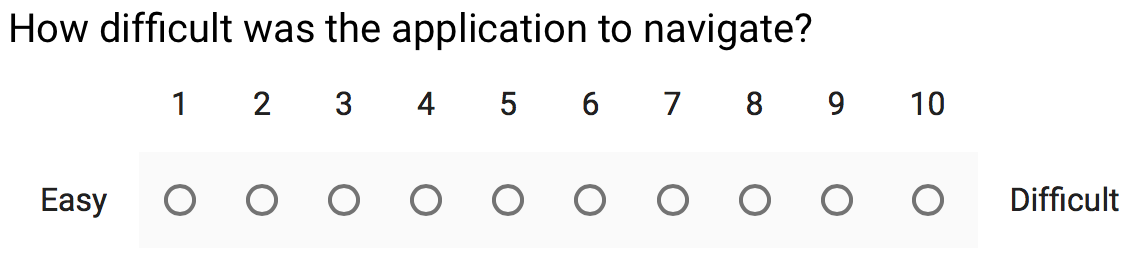
\includegraphics[width=1.0\textwidth]{images/Testing/UA_Difficulty}
	\caption{Questionnaire Regarding System Difficulty} \label{fig:UA_Difficulty}
\end{figure}

Initially the navigation for the system was quite complex and contained many links without any icons. Figure \ref{fig:UA_Difficulty} shows an example question that was presented to the user after the navigation had been built and implemented on several pages. These page were blank but the structure was there and the navigation links pointed to the appropriate pages. Upon reading the feedback, the users gave the navigation quite a high difficulty rating on average and as a result the navigation was simplified by reducing links and adding icons which were common sight.

Acceptance testing played a key role in the development process of the system. Prototypes were built and presented to the user which they evaluated and the feedback from the users was then incorporated into the next iteration of the users. Often a different selection was used to provide an unbiased feedback as existing users would be familiar with the system after previous tests. However, on the final acceptance testing of the complete system, a mix of new and existing users were requested to test the system to see what new users thought about the final product as well as how existing users thought the system had improved

\newpage